% !TeX root = ../main.tex

\chapter{长寿命粒子模型}

长寿命粒子(Long Lived Particle, LLP)是指在探测器内衰变的时间尺度远大于标准模型粒子的寿命的粒子,它的存在是许多新物理模型的预言。
LLP长寿命的物理机制一般是由于它的衰变被禁戒或是被压低,
其中压低可能出于衰变末态粒子的近简并质量谱(nearly-degenerate mass states)或是 LLP 与末态粒子的耦合很小。
由于LLP具有较长的寿命、与标准模型粒子仅存在微弱的相互作用,因此它常被认为是暗物质的候选者。


\section{具体模型}
能够产生长寿命粒子的模型有很多种,在本分析中考虑了三种模型作为信号模型:
隐藏区域(Hidden Sector)模型、超对称(supersymmetry)模型与希格斯中介重子生成模型(Higgs-portal baryogenesis model)。


\subsection{隐藏区域模型}
隐藏区域模型假设了一个由非阿贝尔规范群$SU(3)\times SU(2) \times U(1)$的单重态粒子组成的隐藏区域,
单重态意味着隐藏区域粒子并不携带色荷、同位旋与超荷,因此该隐藏区域粒子与标准模型粒子不发生直接的相互作用,
而是通过希格斯场产生间接相互作用或引力场产生微弱的相互作用。
\cite{hidden_sector}

对于拥有非零真空期望值的隐藏区域的标量场$\phi_p, \,\expval{\phi_p}=v_p \neq 0$,
它会与标准模型希格斯场$\phi_s$发生耦合并形成混合态,其相互作用拉氏量为
\begin{equation}
    \mathcal{L}_\text{link} = \eta \phi^\dagger_s \phi_s \phi^\dagger_p \phi_p
\end{equation}
在各自的真空期望值附近展开($\phi_s = v_s + h_s$,$\phi_p = v_p + h_p$),得到质量混合项
\begin{equation}
    \mathcal{L}_\text{mixing} = 4 \eta v_s v_p h_s h_p
\end{equation}
由此产生的质量本征态$h_1, h_2$为标准模型希格斯粒子$h_s$与隐藏区域的类希格斯(Higgs-like)粒子$h_p$的线性组合。

所以这两个拥有确定质量的粒子既可以通过标准模型希格斯粒子耦合到标准模型粒子上,
又可以通过隐藏区域的类希格斯粒子耦合到隐藏区域的粒子上。
分析中感兴趣的过程为质量介于 \SI{60}{GeV} 至 \SI{1000}{GeV} 类希格斯粒子$h_p$衰变为一对
隐藏区域中质量介于 \SI{5}{GeV} 至 \SI{475}{GeV} 长寿命的中性标量粒子$s$,
之后中性标量粒子$s$通过汤川相互作用(Yukawa coupling)衰变为标准模型正反费米子对。
也即考虑衰变过程$h_p \rightarrow ss \rightarrow f \bar{f} f' \bar{f}'$。

当隐藏区域长寿命的中性标量粒子$s$的质量介于两倍底夸克(b quark)与两倍顶夸克(t quark)之间,
也即 \SI{8.48}{GeV} 至 \SI{344}{GeV} 之间时,其衰变道为 88\% 的$b \bar{b}$、8\% 的$c \bar{c}$ 与 4\% 的$\tau \bar{\tau}$。
当$s$的质量大于两倍顶夸克时,衰变被$t \bar{t}$主导。


\subsection{超对称模型}
标准模型为夸克、轻子、规范玻色子被规范群$SU(3)\times SU(2) \times U(1)$控制的可重整理论。
为了解释等级问题(hierarchy problem),也即引力在 \num{e16} 到 \SI{e18}{GeV} 之间的某个能量与强力、电磁力、弱力统一,
我们需要引入超对称性来将费米子与玻色子结合在一起。

超对称模型引入两个左手征超场的$SU(2)$二重态
$$H_1 = \mqty(H_1^0 \\ H_1^-) \qc H_2 = \mqty(H_2^+ \\ H_2^0) $$
来产生$SU(2) \times U(1)$的自发对称破缺并赋予所有夸克、轻子以及$W^\pm$和$Z^0$质量。
同时每个费米子都有一个玻色子伴侣、每个玻色子都有一个费米子伴侣。
\cite{QFT_Weinberg}

为了防止质子在超对称模型中衰变得太快,通常需要引入R宇称并要求它守恒,R宇称定义为
\begin{equation}
    R = (-1)^{3(B-L)+2S}
\end{equation}
其中$B$为重子数、$L$为轻子数、$S$为自旋量子数。
对于所有的标准模型粒子,$R=1$;对于所有的超对称粒子,$R=-1$。
\cite{SUSY_ATLAS}

当R宇称守恒时,最轻的超对称粒子(lightest supersymmetry particle, LSP)是稳定的,因此LSP是暗物质的候选者。
超对称粒子同时也是LLP的候选者,在近最小超对称(Next-to-Minimal supersymmetry)模型中,
引入了规范单重态手征超场(gauge singlet chiral superfield),它的费米子伴侣singlino因为衰变产物质量近简并而被压低衰变,因此成为长寿命粒子。
\cite{singlino}
在分析中,对产生(pair-produced)的质量介于 \SI{250}{GeV} 至 \SI{2000}{GeV} 的胶微子(gluino)发生衰变,
产生质量 \SI{100}{GeV} 的singlino,singlino继续衰变成标准模型粒子被探测器探测。


\subsection{希格斯中介重子生成模型}
希格斯中介重子生成模型(Higgs-portal baryogenesis model)旨在解释通过弱尺度状态衰变而观察到的正反重子不对称现象。
该模型引入了长寿命单重态粒子$\chi$,它与希格斯玻色子混合并衰变为三个费米子,从而违反了重子数与轻子数守恒。
分析考虑了质量介于 10~GeV 至 100~GeV 之间的$\chi$ ,以及$\chi$ 衰变为轻子和夸克组合的各种模式。

长寿命单重态粒子$\chi$的产生与衰变机制具体如下:
\cite{Cui_2015}

粒子 $\chi$ 的产生机制必须遵循使其成为亚稳态的 $Z_2$ 或更高的对称性,这意味着在 LHC 中 $\chi$ 应成对产生。
我们预期存在至少一个相对较大的耦合项,使得 $\chi$ 能以接近暗物质丰度的形式在宇宙早期热冻结(thermally freeze out),
从而可以通过反演其湮灭图得到它的产生方式,并且该产生方式在对撞机中有可观的产率。
作为马约拉纳费米子(Majorana fermion),$\chi$ 要么是标准模型的单重态,要么属于标准模型规范群的实表示。

考虑规范单重态的新亚稳态粒子 $\chi$,它的产生高度依赖于模型结构。
我们类比暗物质研究中的处理方式,将 $\chi$ 的产生按其与标准模型的有效相互作用进行分类。最低维有效算符如下:
\begin{equation}
    \mathcal{L}_{\text{prod}}^{\text{singlet}} \supset \frac{c_H}{\Lambda_H} \chi^2 |H|^2 +
    \frac{c_q}{\Lambda_q^2} (\bar{\chi} \Gamma \chi)(\bar{q} \Gamma' q) +
    \frac{c_g}{\Lambda_g^3} \chi^2 (G_{\mu\nu})^2 + \cdots
\end{equation}
其中第一项为希格斯中介(Higgs portal),第二项为经由狄拉克矩阵$\Gamma, \Gamma'$与夸克进行耦合,第三项为胶子中介(gluon portal)。
为具体起见,我们聚焦于最低维的希格斯中介耦合,其他算符导致类似的对撞机现象,只是产生率有所不同。

与由 $Z_2$ 守恒相互作用主导的产生过程不同,$\chi$ 的衰变由 $Z_2$ 破缺相互作用引发。
$\chi$ 的衰变违反重子数和/或轻子数守恒,此类相互作用的最低维允许 $\chi$ 衰变为三个标准模型费米子。
我们将所有可与 $\chi$ 耦合的三费米子标准模型算符进行分类如下:
\begin{itemize}
    \item {标记为 $q$ 的算符:} 至少包含两个夸克;
    \item {标记为 $\ell$ 的算符:} 仅包含轻子;
    \item {标记为 $L$ 的算符:} 含两个 $SU(2)_L$ 左手双重态;
    \item {标记为 $R$ 的算符:} 仅包含 $SU(2)_L$ 右手单重态。
\end{itemize}
得到有效拉氏量形式为:
\begin{equation}
    \mathcal{L}_{\text{decay}} \supset \chi (\mathcal{O}, \mathcal{O}^\dagger) + \text{h.c.}
\end{equation}
其中可能的算符$\mathcal{O}$包括:
\begin{itemize}
    \item $\mathcal{O}_{qL}     : \lambda'_{ijk} Q_i D_j L_k,\quad \eta'_{ijk} Q_i U_j L^\dagger_k,\quad \eta''_{ijk} Q_i Q_j d^\dagger_k$
    \item $\mathcal{O}_{qR}     : \lambda''_{ijk} U_i D_j D_k,\quad \eta_{ijk} U_i E_j D^\dagger_k$
    \item $\mathcal{O}_{\ell L} : \lambda_{ijk} L_i L_j E_k$
\end{itemize}

若 $\chi$ 为单重态,则可耦合所有上述算符;若 $\chi$ 属于规范群的伴随表示,则其耦合仅限于可与该规范群基本表示场耦合的算符。
例如,$SU(3)$ 八重态(如 gluino)可耦合 $\mathcal{O}_{qL}$ 和 $\mathcal{O}_{qR}$,
$SU(2)_L$ 三重态(如 wino)可耦合 $\mathcal{O}_{qL}$ 和 $\mathcal{O}_{\ell L}$。


\section{探测器特征}
由于LLP能在衰变前行进一定的宏观距离,其衰变产物不会从原始碰撞点(Primary Vertices)产生,
而是在远离大多数标准模型粒子产生的初级顶点处形成一个次级顶点(Secondary Vertices),该顶点也被称为偏离对撞顶点(Displaced Vertices)。
进一步,当LLP的衰变位置在电磁量能器之后时,其衰变产物会在电磁量能器内沉积少量能量,并且在其后的强子量能器内沉积绝大部分能量。
通过定义喷注在两类量能器中沉积的能量比值$$\text{CalRatio}=E_{\text{H}}/E_{\text{EM}}$$
其中$E_{\text{H}}$为强子量能器内沉积的能量、$E_{\text{EM}}$电磁量能器内沉积的能量,可以作为鉴别LLP的衰变的重要参数。
\cite{calratio}

尽管目标LLP是在强子量能器中才发生衰变,但我们仍预期在电磁量能器中会有少量的能量沉积,原因有二。
其一是本分析对于在电磁量能器的后端发生衰变的LLP仍然敏感,该情况同样会导致较高的 CalRatio 值。
其二是由于一些与信号无关的现象可能会导致在电磁量能器中沉积能量。

\begin{figure}[ht]
    \centering
    \hfill
    \subfloat[真实数据、BIB数据与信号数据的$\log_{10}\text{CalRatio}$分布图]
    {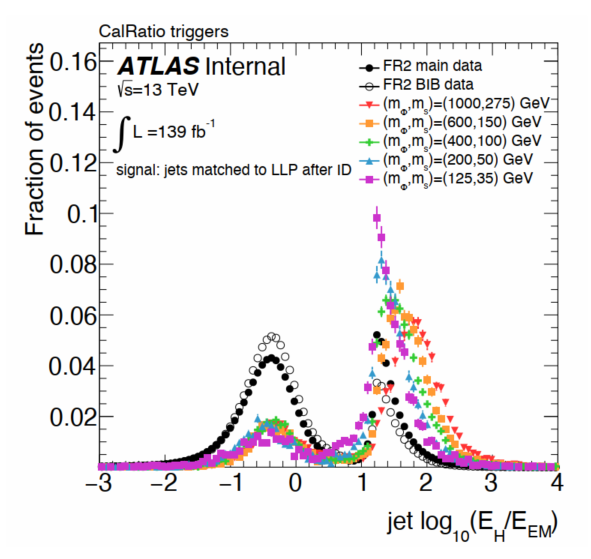
\includegraphics[width=0.43\textwidth]{CalRatioDistribution_1.png}}
    \hfill
    \subfloat[信号数据的$\log_{10}\text{CalRatio}$关于$L_{xy}$的分布图]
    {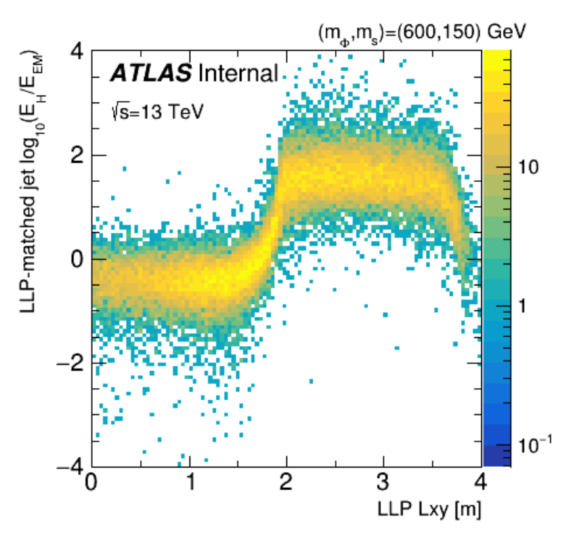
\includegraphics[width=0.43\textwidth]{CalRatioDistribution_2.png}}
    \hfill
    \caption{CalRatio分布图\cite{ATLAS:2022zhj}}
    \label{fig:CalRatioDistribution}
    \figurenote{
        注:束流背景(Beam Induced Background,BIB)为本分析感兴趣的背景之一
    }
\end{figure}

从\autoref{fig:CalRatioDistribution} 的(a)图可以看出,
LLP 的信号数据在$\log_{10}\text{CalRatio}$分布上与真实数据和背景数据有明显的区别,
在$-1.5<\log_{10}\text{CalRatio}<0.5$的区间背景数据分布比例高而信号数据分布比例低,
而在$1<\log_{10}\text{CalRatio}<2.5$的区域背景数据分布比例低而信号数据分布比例高。
\autoref{fig:CalRatioDistribution} 的(b)图则是 LLP 在不同的$x$--$y$平面衰变位置$L_{xy}$下$\log_{10}\text{CalRatio}$的分布,
其中筒部的电磁量能器位于$\SI{1.5}{m} < L_{xy} < \SI{2}{m}$处、强子量能器位于$\SI{2}{m} < L_{xy} < \SI{4}{m}$处,
所以在$L_{xy} > \SI{2}{m}$时LLP的衰变产物会显著减少在电磁量能器内沉积的能量,因而能观察到$\log_{10}\text{CalRatio}$显著增加。

\begin{figure}[ht]
    \centering
    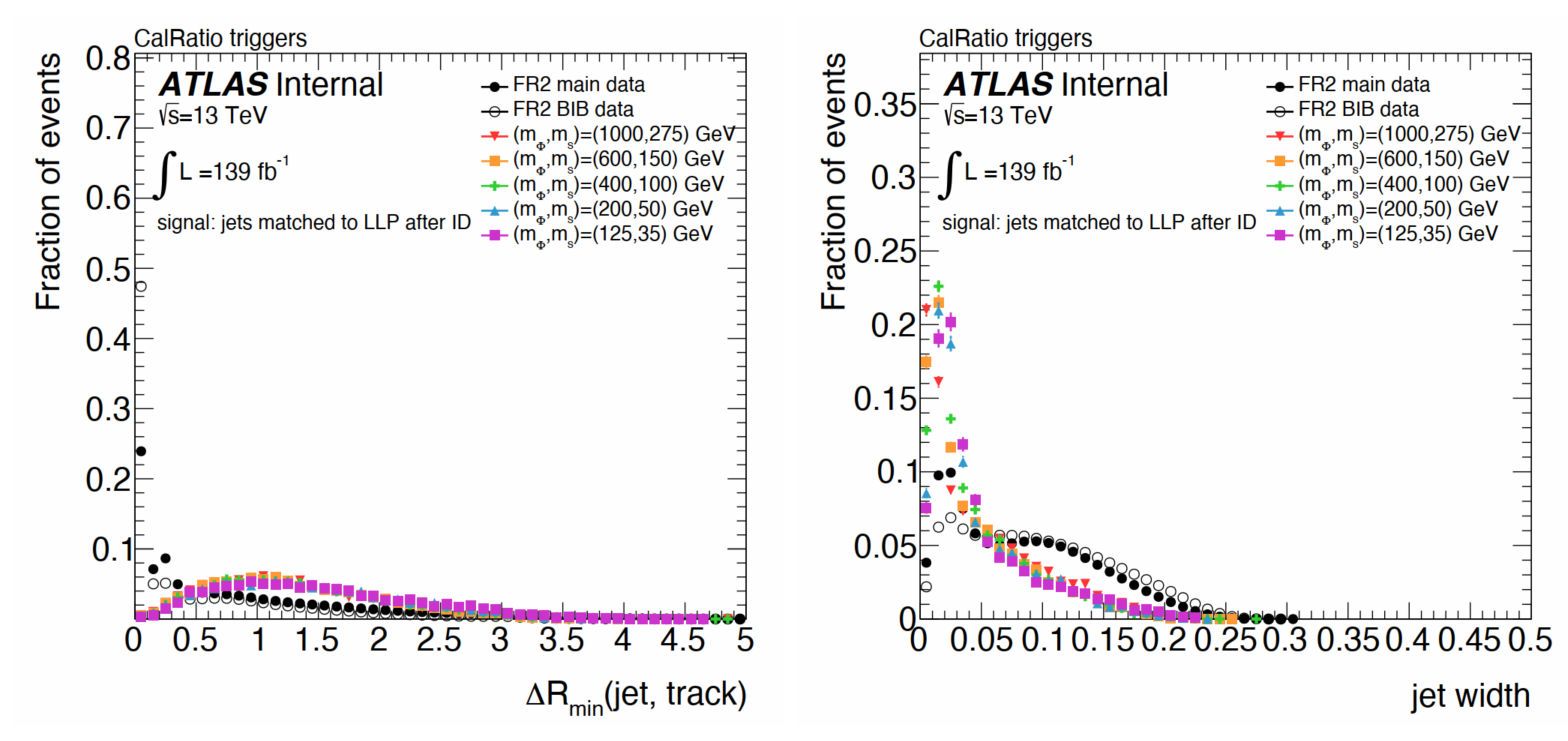
\includegraphics[width=0.85\textwidth]{DR_jet_width.png}
    \caption{$\Delta R_{\min}$与喷注宽度的分布图\cite{ATLAS:2022zhj}}
    \label{fig:DR_jet_width}
    \figurenote{
        左图:喷注中$p_T>\SI{2}{GeV}$的径迹距离喷注轴线方向的最小角距离的分布图,角距离$\Delta R = \sqrt{(\Delta \phi)^2+(\Delta \eta)^2}$;
        右图:喷注宽度的分布图,喷注宽度定义为
        $\sum_{i \in \text{tracks}} p_{\text{T}, i} \Delta R_i / \sum_{i \in \text{tracks}} p_{\text{T}, i}$,
        即以\pt 加权的径迹与喷注轴线的角距离。
    }
\end{figure}

由于感兴趣的 LLP 的衰变发生在量能器而非初级顶点,喷注中的粒子能够在探测器中扩散的时间与距离减少,导致喷注宽度变小。
从\autoref{fig:DR_jet_width} 可以看出相较于LLP衰变产生的喷注,标准模型的喷注可能有部分更靠近轴线方向的次级粒子,
但考虑所有喷注的贡献后,它的最小角距离和 $\sum \Delta R_{\text{min}}(\text{jet, tracks})$ 是更大的。

最小角距离和 $\sum \Delta R_{\text{min}}(\text{jet, tracks})$ 的计算方式为:
考虑一个喷注中满足特定条件(详见\autoref{sec:jet_preselection})的所有径迹,
用 $\Delta R_{\text{min}}(\text{jet, tracks})$ 表示该喷注轴线到它们的角距离
$R = \sqrt{(\Delta \phi)^2 + (\Delta \eta)^2}$ 的最小值。
随后,将事件中满足 \(p_T > 50~\text{GeV}\) 的 clean 喷注(筛选条件见\autoref{sec:jet_preselection})的
\(\Delta R_{\text{min}}(\text{jet, tracks})\) 求和,
得到 \(\sum \Delta R_{\text{min}}(\text{jet, tracks})\) 的值。

综上所述,我们可以通过物理量诸如CalRatio与$\sum \Delta R_{\text{min}}(\text{jet, tracks})$来区分LLP产生的喷注与标准模型的喷注。
该思想将被运用到数据获取的触发与后续的分析中。
